\documentclass{beamer}
\usepackage{graphics}
\usepackage{blindtext}
\usepackage{fancybox}
\usepackage{tikz}
\usepackage{caption}
\usepackage[backend=bibtex, style=numeric, sorting=none]{biblatex}
\addbibresource{/home/gaurish108/Dropbox/MyWiki/research_projects/HorseFly/writeups/horsefly_refs.bib}
\newcommand*{\rom}[1]{\expandafter\@slowromancap\romannumeral #1@}

\usetheme[progressbar=frametitle]{metropolis}
\useoutertheme{metropolis}
\useinnertheme{metropolis}
\usefonttheme{metropolis}
%\usecolortheme{spruce}
\setbeamercolor{background canvas}{bg=white}

\date{}
\title{Package Delivery with Trucks and Drones: The Horsefly Problem}
\subtitle{}
\author{Joseph S. B. Mitchell, \hspace{2pt} Gaurish Telang}
\institute{ \vspace{-8pt} Stony Brook University, New York \\\vspace{9pt}
{\textit{\tiny(In collaboration with John Gunnar Carlsson, S\'andor Fekete, and Sujoy Bhore)}}  \\ \\ Fall Workshop in Computational Geometry, 2018 \\ }
\begin{document}
\metroset{block=fill}


%%%%%%%%%%%%%%%%%%%%%%%%%%%%%%%%%%%%%%%%%%%%%%%%%%%%%%%%%%%%%%%%%%%%%%%%%%%%%%%%%%%%%%%%%%%%%%%%%%
\begin{frame}
  \titlepage
  In collaboration with SJohn Gunnar Carlsson, Sandor Fekete, and Sujoy Bhore
\end{frame}
%%%%%%%%%%%%%%%%%%%%%%%%%%%%%%%%%%%%%%%%%%%%%%%%%%%%%%%%%%%%%%%%%%%%%%%%%%%%%%%%%%%%%%%%%%%%%%%%%%
% For the most part follow the presentation given 
% in the FWCG submission. Throw in a few interesting
% examples for good measure, along with conjectures,
% future-work yada, yada. When no obstacles involved
% point out that a realistic setting would involve
% obstacles, or road=network...Add to last section
% maybe? 
\begin{frame}[t]{Using Trucks and Drones in Tandem}
  \begin{columns}
    \begin{column}{0.45\textwidth}
      \begin{figure}
        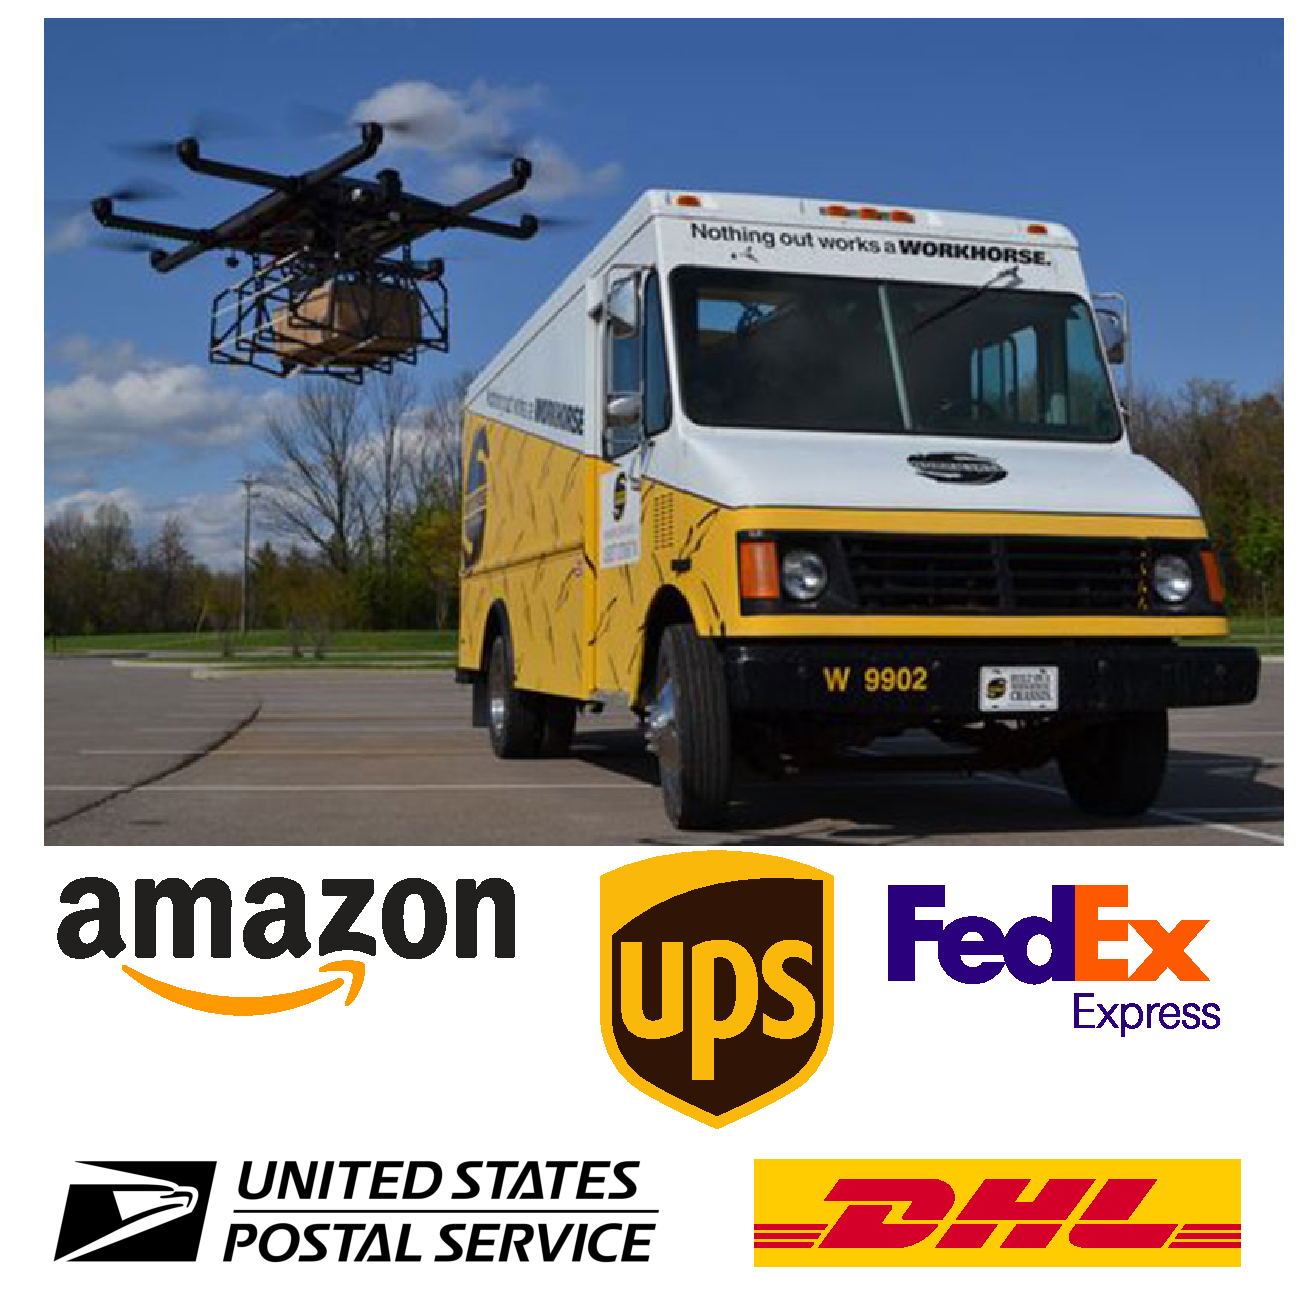
\includegraphics[width=6.0cm]{slide_imgs/introslide_image.eps}
      \end{figure}
    \end{column}

    \begin{column}{0.55\textwidth}
      \vspace{25pt}
      \begin{quote}
      ``UPS has estimated
  that cutting off just one mile for the routes of each of the
  company's 66,000 delivery drivers would amount to   {\color{red}   \$50 million } in
  savings. For this reason, UPS is testing drone deliveries, using the
  top of its vans as a mini-helipad.'' \footnotemark
  \end{quote}
    \end{column}
  \end{columns}
 \vspace{2mm}
  \footnotetext[1]{ From \url{https://www.businessinsider.com/amazon-and-ups-are-betting-big-on-drone-delivery-2018-3}}
\end{frame}

%%%%%%%%%%%%%%%%%%%%%%%%%%%%%%%%%%%%%%%%%%%%%%%%%%%%%%%%%%%%%%%%%%%%%%%%%%%%%%%%%%%%%%%%%%%%%%%%%%

\begin{frame}{Statement of Horsefly-PATH}
  \begin{columns}
    \begin{column}{0.5\textwidth}
    % A sample image dscribing horsefly path
    \vspace{-19pt}
    \begin{figure}
      \only<1>{\includegraphics[width=6cm]{slide_imgs/horsefly_demo_input.jpg}}
      \only<2>{\includegraphics[width=6cm]{slide_imgs/horsefly_demo_output.jpg}}
    \end{figure}
    
    {\small
      \vspace{-15pt}
      \definecolor{dronegreen}{rgb}{0.0, 0.5, 0.0}
      \hspace{40pt} Speed Ratio \varphi = 3.0 \\
      \hspace{40pt} Truck Path : \tikz[baseline=-0.5ex]{ \draw[red, thick] [-] (0,0) -- (5ex,0); }  \\
      \hspace{40pt} Drone Path : \tikz[baseline=-0.5ex]{ \draw[dronegreen, thick] [-] (0,0) -- (5ex,0); }  \\
     } 
    \end{column}

    \begin{column}{0.5\textwidth}
      \begin{center}
        Compute a route for the truck and for the drone in order to complete the delivery of
        all $n$ packages (and have the drone return back to the empty truck)
        was soon as possible i.e., we seek to {\color{red} minimize  makespan} of the delivery process.
        
        {\tiny Both the {\color{red} order} of visiting the sites \underline{and} {\color{red} Steiner points} need to be computed!}
        \end{center}
    \end{column}
    
  \end{columns}
\end{frame}


%%%%%%%%%%%%%%%%%%%%%%%%%%%%%%%%%%%%%%%%%%%%%%%%%%%%%%%%%%%%%%%%%%%%%%%%%%%%%%%%%%%%%%%%%%%%%%%%%%%%%%%

\begin{frame}{Preliminary Notes}
    \begin{columns}
    \begin{column}{0.5\textwidth}
      % A sample image dscribing horsefly path
      \vspace{-19pt}
    \begin{figure}
      \includegraphics[width=6cm]{slide_imgs/horsefly_demo_output.jpg}
    \end{figure}

    
    {\small
      \vspace{-15pt}
      \definecolor{dronegreen}{rgb}{0.0, 0.5, 0.0}
      \hspace{40pt} Speed Ratio \varphi = 3.0 \\
      \hspace{40pt} Truck Path : \tikz[baseline=-0.5ex]{ \draw[red, thick] [-] (0,0) -- (5ex,0); }  \\
      \hspace{40pt} Drone Path : \tikz[baseline=-0.5ex]{ \draw[dronegreen, thick] [-] (0,0) -- (5ex,0); }  \\
     } 
    \end{column}

   \begin{column}{0.5\textwidth}
      \begin{itemize}
       \item[(1)] Horsefly is {\color{red} NP-complete}, by reduction from TSP ($\varphi = 1.0$)
       \item[(2)] Truck or drone {\color{red} never wait} in OPT for Horsefly-PATH. 
       \item[(3)] The truck route and the drone route are {\color{red} polygonal}
       \item[(4)] The truck and the drone move always at their {\color{red} maximum speeds}(1 and $\varphi$, respectively).
      \end{itemize}
    \end{column}
    
  \end{columns}
       
\end{frame}


%%%%%%%%%%%%%%%%%%%%%%%%%%%%%%%%%%%%%%%%%%%%%%%%%%%%%%%%%%%%%%%%%%%%%%%%%%%%%%%%%%%%%%%%%%%%%%%%%%
% Place a TikZ pictures.
\begin{frame}{Preliminary Notes: Optimal Order depends on $\varphi$}
  \begin{center}

    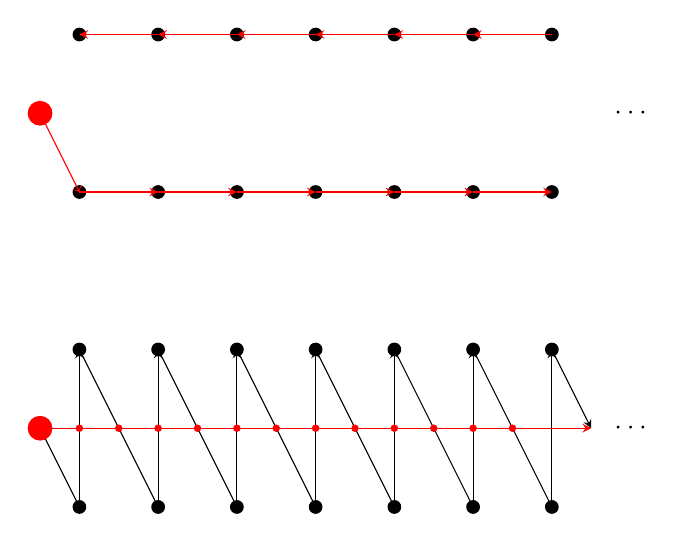
\begin{tikzpicture}
      %%%%%%%%%%%%%%%%%%%%%%%%%%%%%%%%%%%%%%%%%%%%%%
      %%% When speed ration is 1.0, follow TSP path
      %%%%%%%%%%%%%%%%%%%%%%%%%%%%%%%%%%%%%%%%%%%%%
     \foreach \x in {0,...,6} % top row of sites
         \draw[fill] (\x,4) circle (0.08cm);
     \foreach \x in {0,...,6} % bottom row of sites
         \draw[fill] (\x,6) circle (0.08cm);
     % Path of the horse. Draw it as red.
     \foreach \x in {0,...,5}
          \draw [->, red , >=stealth]  (\x,4) -- (\x+1,4); 
          
     \foreach \x in {0,...,5}
          \draw [<-, red , >=stealth]  (\x,6) -- (\x+1,6); 
      % Path of the drone
      \draw [->, red] (-0.5,5) -- (0,4);

     % Assume there are lots of sites to the right
     \node[draw=none] (ellipsis1) at (7,5) {$\cdots$};

     % Initial position of the horse and fly.
     \draw[fill, red] (-0.5,5) circle (0.15cm); 

      %%%%%%%%%%%%%%%%%%%%%%%%%%%%%%%%%%%%%%%%%%
      %%% When speed ratio is not 1.0
      %%%%%%%%%%%%%%%%%%%%%%%%%%%%%%%%%%%%%%%%%%
     \foreach \x in {0,...,6} % top row of sites
         \draw[fill] (\x,0) circle (0.08cm);
     \foreach \x in {0,...,6} % bottom row of sites
         \draw[fill] (\x,2) circle (0.08cm);
      % Path of the drone
      \draw [->] (-0.5,1) -- (0,0);
      \foreach \x in {0,...,6}
          \draw [->, >=stealth]  (\x,0) -- (\x,2);    
      \foreach \x in {0,...,5}
          \draw [->]  (\x,2) -- (\x+1,0); 
      \draw [->, >=stealth] (6,2) -- (6.5,1); 
      % Rendezvous points
      \foreach \x in {0,...,5}
      {\draw [fill, red]  (\x,1) circle (0.04cm);
        \draw [fill, red]  (\x+0.5,1) circle (0.04cm);
      }
      % Initial position of the horse and fly.
     \draw[fill, red] (-0.5,1) circle (0.15cm); 
      % Path of the horse
     \draw[->, red, >=stealth] (-0.5,1) -- (6.5,1) ;
     % Assume there are lots of sites to the right
     \node[draw=none] (ellipsis1) at (7,1) {$\cdots$};

   \end{tikzpicture}

   
   \end{center}

  
\end{frame}

%%%%%%%%%%%%%%%%%%%%%%%%%%%%%%%%%%%%%%%%%%%%%%%%%%%%%%%%%%%%%%%%%%%%%%%%%%%%%%%%%%%%%%%%%%%%%%%%%%

\begin{frame}[fragile]{Preliminary Notes: Optimal Order depends on $\varphi$}
  \vspace{-10pt}
  \begin{figure}
    \centering
    \includegraphics[width=6cm]{slide_imgs/frame-exact-00000.png}
  \end{figure}

\vspace{-15pt} 
\definecolor{coolgrey}{rgb}{0.55, 0.57, 0.67}
{\color{coolgrey} {\tiny 
  \begin{verbatim}
   Show Movie: gnome-open output-exact.mp4&
  \end{verbatim} } }
  
\end{frame}

%%%%%%%%%%%%%%%%%%%%%%%%%%%%%%%%%%%%%%%%%%%%%%%%%%%%%%%%%%%%%%%%%%%%%%%%%%%%%%%%%%%%%%%%%%%%%%%%%%
% Some heuristics and algorithms along
% with conjectured guarantees. Mention
% the scheme based on building trees
% bottom-up which works for arbitrary numbers
% of drones? 

\begin{frame}{An $O(\log n)$ approximation}
\end{frame}

%%%%%%%%%%%%%%%%%%%%%%%%%%%%%%%%%%%%%%%%%%%%%%%%%%%%%%%%%%%%%%%%%%%%%%%%%%%%%%%%%%%%%%%%%%%%%%%%%%
\begin{frame}{When Order of Visitation is Given (Exact Solution)}
  \vspace{-25pt}
  \begin{figure}[H]
    \centering
    \includegraphics[width=10.5cm]{../img/lpdescr.pdf}
  \end{figure}
  \vspace{-10pt}
  $$\displaystyle \min_{(p_0,p_1,\ldots,p_{2n-1}) \in \mathbb{R}^{2n}}  \sum_{i=1}^{n}  || P_i - P_{i-1} ||$$

\vspace{-7pt}
subject to \(n\) constraints \\

\hspace{40pt}$||P_{i}-P_{i-1}||=\frac{ || P_{i-1}-S_{i}|| + ||S_{i}-P_{i}||}{\varphi}\qquad \text{for} \;\; i \in \{1,2,\ldots n\}$
\end{frame}

%%%%%%%%%%%%%%%%%%%%%%%%%%%%%%%%%%%%%%%%%%%%%%%%%%%%%%%%%%%%%%%%%%%%%%%%%%%%%%%%%%%%%%%%%%%%%%%%%%

\begin{frame}{When Order of Visitation is Given (LP Approximation)}
  \vspace{-25pt}
  \begin{figure}[H]
    \centering
    \includegraphics[width=10.5cm]{../img/lpdescr.pdf}
  \end{figure}
  \vspace{-10pt}
  $$\displaystyle \min_{(p_0,p_1,\ldots,p_{2n-1}) \in \mathbb{R}^{2n}}  \sum_{i=1}^{n}  || P_i - P_{i-1} ||$$

\vspace{-7pt}
subject to \(n\) constraints \\

\hspace{40pt}$||P_{i}-P_{i-1}||=\frac{ || P_{i-1}-S_{i}|| + ||S_{i}-P_{i}||}{\varphi}\qquad \text{for} \;\; i \in \{1,2,\ldots n\}$
\end{frame}

\begin{frame}[t]{Exact Solution vs. LP Approximation: An Example}
  \begin{columns}
    \begin{column} {0.5\textwidth}
      \begin{figure}
        \includegraphics[width=6.0cm]{../img/Greedy_SLSQP.pdf}
      \end{figure}
    \end{column}

    \begin{column}{0.5\textwidth}
       \begin{figure}
        \includegraphics[width=6.0cm]{../img/Greedy_LP.pdf}
      \end{figure}
     \end{column}
   \end{columns}
\end{frame}

%%%%%%%%%%%%%%%%%%%%%%%%%%%%%%%%%%%%%%%%%%%%%%%%%%%%%%%%%%%%%%%%%%%%%%%%%%%%%%%%%%%%%%%%%%%%%%%%%%

\begin{frame}{Exact Solution vs. LP Approximation}
  \begin{figure}
        \includegraphics[width=10.0cm]{../img/tour_length_ratios.png}
        \caption*{Conjectured Worst-case Approximation Ratio of LP to SLSQP: {$\sqrt{2} \; o(\varphi) $}}
  \end{figure}
\end{frame}

%%%%%%%%%%%%%%%%%%%%%%%%%%%%%%%%%%%%%%%%%%%%%%%%%%%%%%%%%%%%%%%%%%%%%%%%%%%%%%%%%%%%%%%%%%%%%%%%%%

\begin{frame}{A Special Case: Collinear Horseflies}
  \vspace{-10pt}
 \begin{figure}[H]
    \centering
    \includegraphics[width=6.0cm]{../img/collinear_horseflies.png}
  \end{figure}

\end{frame}

%%%%%%%%%%%%%%%%%%%%%%%%%%%%%%%%%%%%%%%%%%%%%%%%%%%%%%%%%%%%%%%%%%%%%%%%%%%%%%%%%%%%%%%%%%%%%%%%%%
\begin{frame}{Greedy Heuristic (1) : Go to Nearest Unserviced Site }
\end{frame}

%%%%%%%%%%%%%%%%%%%%%%%%%%%%%%%%%%%%%%%%%%%%%%%%%%%%%%%%%%%%%%%%%%%%%%%%%%%%%%%%%%%%%%%%%%%%%%%%%%
\begin{frame}{Greedy Heuristic (2) : Cheapest Insertion }
\end{frame}

%%%%%%%%%%%%%%%%%%%%%%%%%%%%%%%%%%%%%%%%%%%%%%%%%%%%%%%%%%%%%%%%%%%%%%%%%%%%%%%%%%%%%%%%%%%%%%%%%%
\begin{frame}{K2means Heuristic}
   \begin{figure}[H]
    \centering
    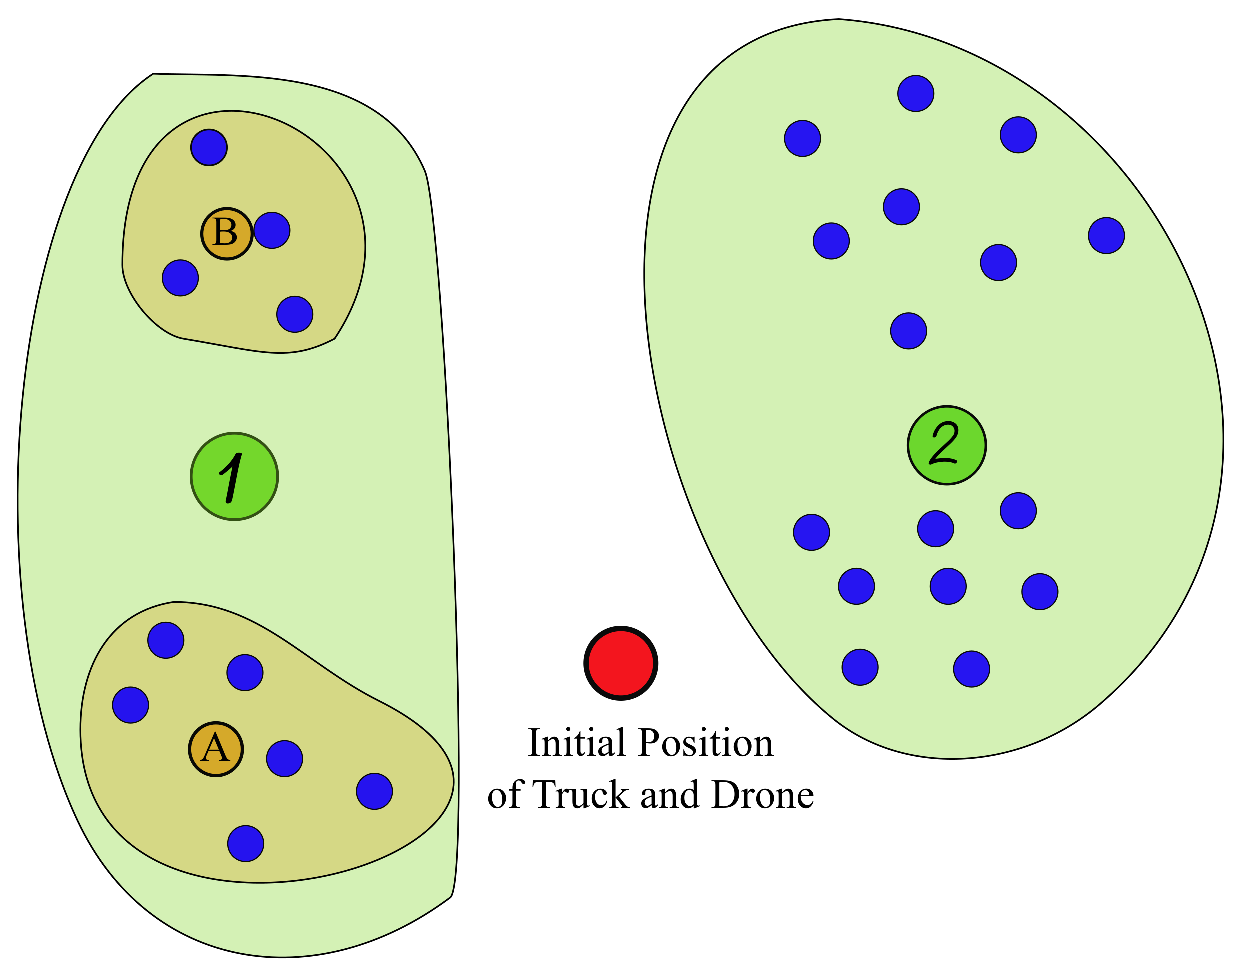
\includegraphics[width=8.0cm]{../img/k2means_explain.eps}
  \end{figure}

\end{frame}
%%%%%%%%%%%%%%%%%%%%%%%%%%%%%%%%%%%%%%%%%%%%%%%%%%%%%%%%%%%%%%%%%%%%%%%%%%%%%%%%%%%%%%%%%%%%%%%%%%
\begin{frame}{Comparing Greedy Heuristic (1) and K2means heuristic}
 \begin{columns}
    \begin{column} {0.5\textwidth}
      \begin{figure}
        \includegraphics[width=6.0cm]{../img/greedy_example.pdf}
      \end{figure}
    \end{column}

    \begin{column}{0.5\textwidth}
       \begin{figure}
        \includegraphics[width=6.0cm]{../img/k2means_example.pdf}
      \end{figure}
     \end{column}
   \end{columns}

\end{frame}

\section{Ongoing and future work}

\begin{frame}{Variants: Reverse Horsefly}
  \begin{figure}
    \centering
        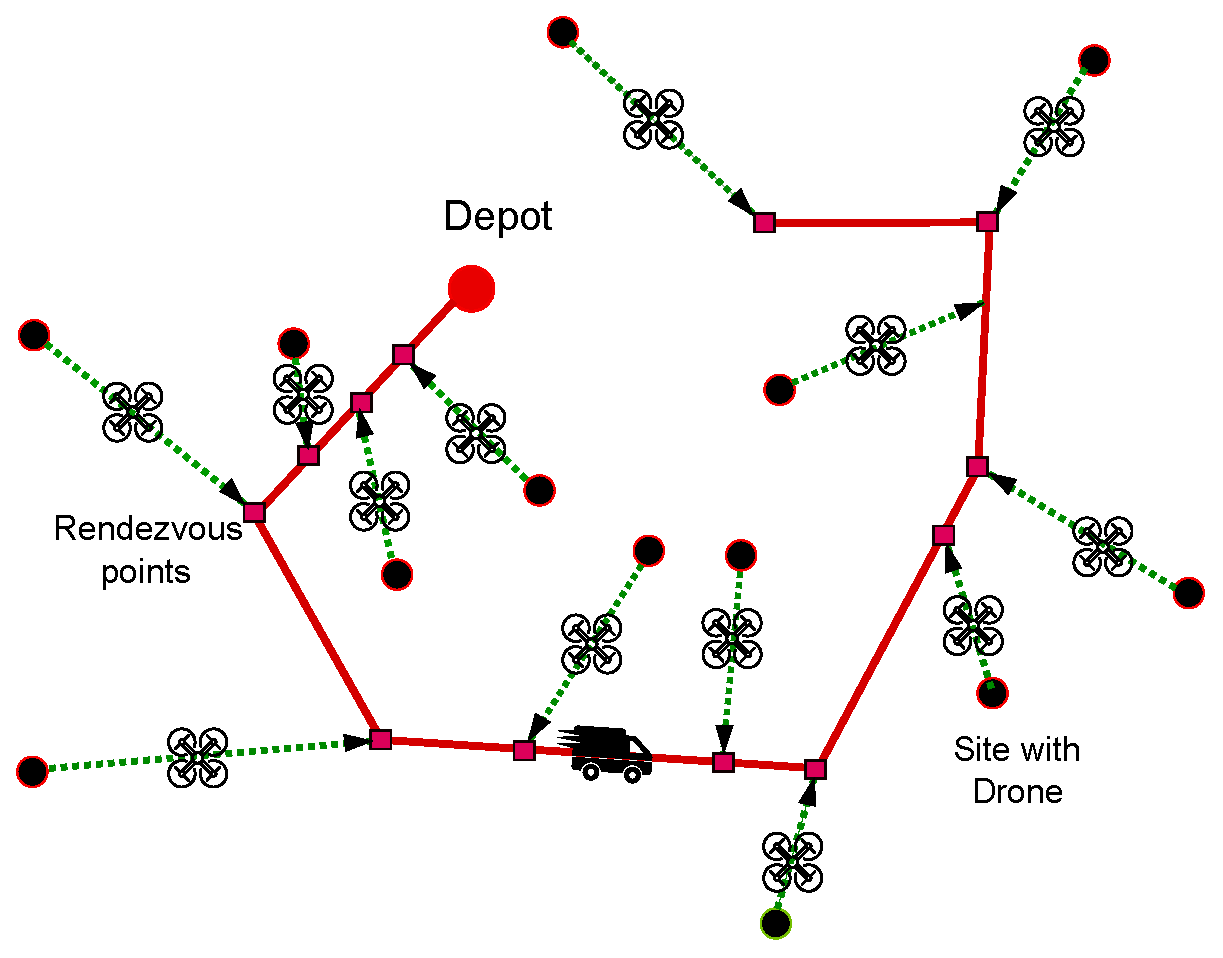
\includegraphics[width=10.0cm]{slide_imgs/reverse_horsefly.eps}
  \end{figure}

\end{frame}

\begin{frame}{Variants: Fixed Truck Route}
\begin{figure}
    \centering
        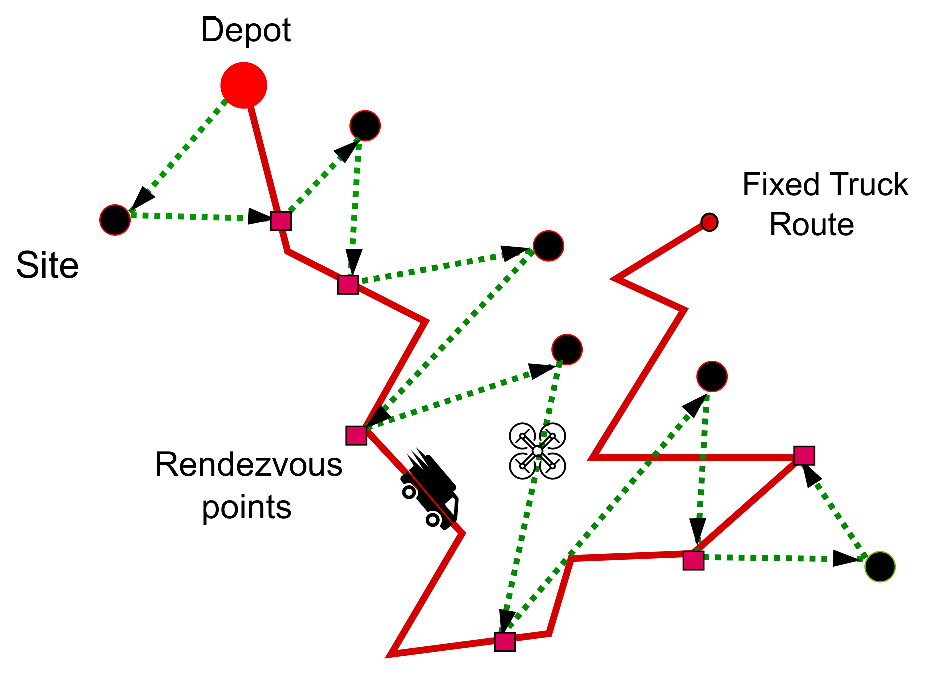
\includegraphics[width=8.0cm]{slide_imgs/fixed_truck_route_variant.eps}
  \end{figure}

\end{frame}


\begin{frame}{Variants: Segment Horsefly}
\begin{figure}
    \centering
        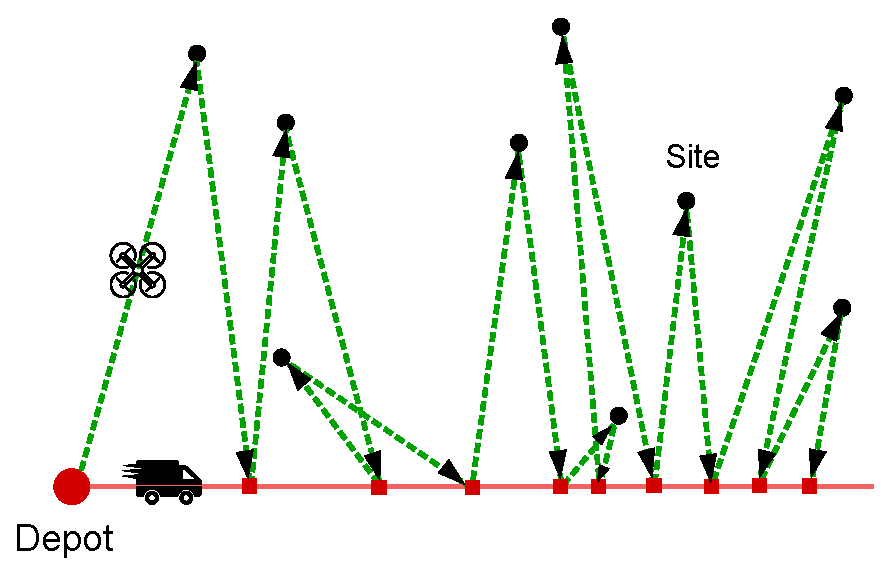
\includegraphics[width=10.0cm]{slide_imgs/segment_horsefly.eps}
  \end{figure}

\end{frame}

\begin{frame}{Variants: Multiple Drones}
\end{frame}





\end{document}